\chapter{The CMS Detector at the Large Hadron Collider}

The CMS detector is a general purpose particle detector which measures the energy and momentum of particles produced in the collision of high energy protons in the Large Hadron Collider at CERN \cite{collaborationCMSExperimentCERN2008}. It was designed with the goal of studying a wide range of physics phenomena, including the study of the electroweak sector, vector boson scattering, precision studies of the standard model (SM), heavy-ion physics, and searches for beyond the SM physics. The CMS detector is cylindrical, with an overall diameter of $15.0 \text{ m}$, a length of $28.7 \text{ m}$ and a total weigtht of $14,00\text{ m}$. A schematic of the CMS detector is shown in Figure \ref{fig:cms_detector}.

\begin{figure}[ht]
	\centering
	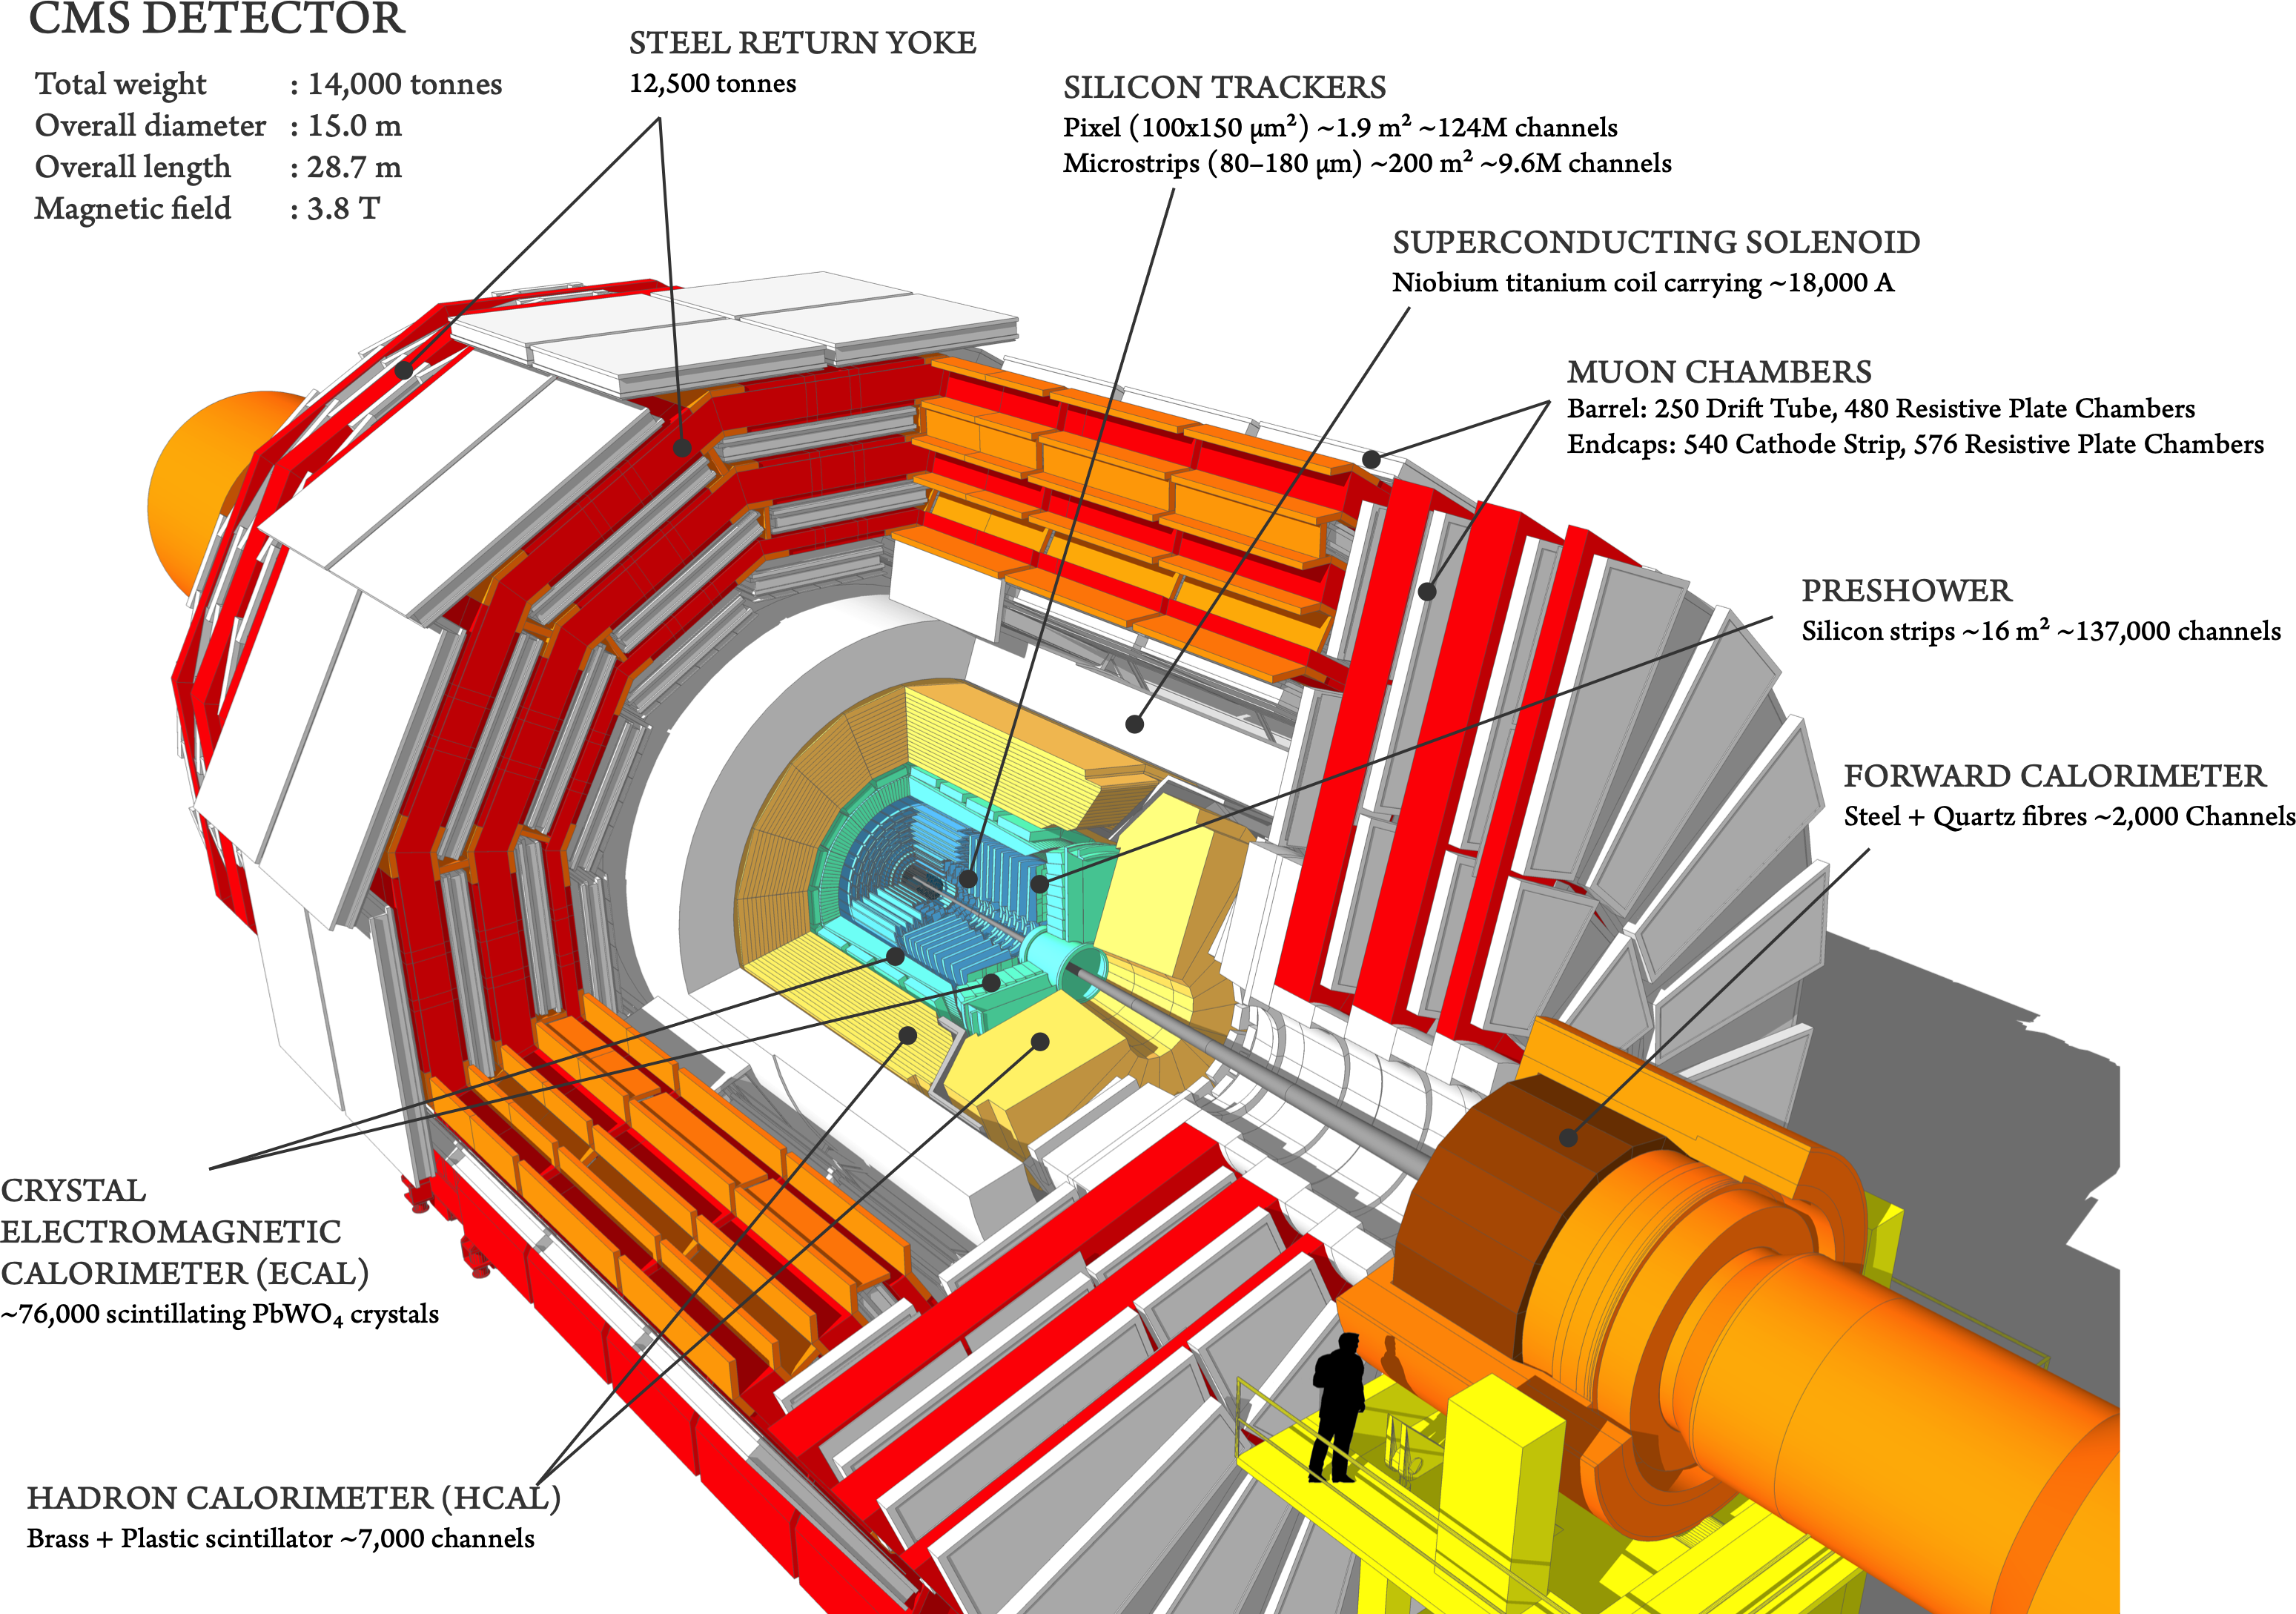
\includegraphics[width=0.8\textwidth]{images/cms_detector.png}
	\caption{Schematic of the CMS detector at the Large Hadron Collider.}
	\label{fig:cms_detector}
\end{figure}

This chapter will provide an overview of the CMS detector, with a subsequent particular focus on the Run 3 upgrades to the calorimeters as well as the trigger system and the novel trigger strategies that have been developed in the search for new physics.

\section{Detector Overview}

\section{Run 3 Upgrades}

\section{Trigger System}
